\chapter{Unfallerkennung im Pocket-Mode}

- Unterschied zum aktuellen Ziel:\\
- Smartphone wird momentan am Lenker befestigt\\

Konkreter Unterschied zu meiner MA

\section{Kritische Unfallszenarien}

Liste der Edge- und usecases mit einer Erklärung, warum diese kritisch sind und einen Vorschlag, was man dagegen tun kann.



\section{Lauferkennung} \label{sec:Lauferkennung}

%\begin{table}\caption{Statistische Zahlen über Unfälle in Deutschland \cite{Verkehrsunfaelle_Fahrrad2017}} 
%	\centering
%	\begin{tabular}{|p{3.2cm}|>{\centering\arraybackslash}p{3.3cm}|>{\centering\arraybackslash}p{3.3cm}|>{\centering\arraybackslash}p{3.3cm}|}
	%		\hline
	%		\textbf{Jahr} & \textbf{Unfälle} & \textbf{Verunglückte} & \textbf{Getötete} \\
	%		\hline
	%		2000 & 382.949 & 511.577 & 7.503 \\
	%		\hline
	%		2005 & 336.619 & 438.804 & 5.361 \\
	%		\hline
	%		2010 & 288.297 & 374.818 & 3.648 \\
	%		\hline
	%		2014 & 302.435 & 392.912 & 3.377 \\
	%		\hline
	%		2015 & 305.659 & 396.891 & 3.459 \\
	%		\hline
	%		2016 & 308.145 & 399.872 & 3.206 \\
	%		\hline
	%		2017 & 302.656 & 393.492 & 3.180 \\
	%		\hline
	%	\end{tabular}
%	\label{tab:UnfallImJahren}
%\end{table}
%
\subsection{Peaks aufzählen} %TODO: ausführlich beschreiben
1. Idee:\\

Einen Zähler zu implementieren. Das soll alle Peaks aufzählen mit der Hoffnung, dass es Unterschied zwischen Laufen und Fahren zu erkennen ist.
Das LaufFrequenz ist zwischen 0.5-4 Hz. Das Fahren ist über 20 Hz.
Es wurde einen Testbeispiel mit einem Sinussignal gebaut und das Prinzip getestet.
\begin{figure}[H]
	\centering
	\includegraphics[width=\linewidth]{Bilder/Lauferkennung_Peaks_Testbeispiel.png}
	\caption{Testbeispiel - Lauferkennung - Peaks Zähler}
	\label{fig:Lauferkennung_Peaks_Testbeispiel}
\end{figure}

In der \autoref{fig:Lauferkennung_Peaks_Testbeispiel} ist das Beispielmodell zur Lauferkennung basiert auf das Zählen jedes Peak des Signals. Im Modell wurde ein Sinussignal generiert (\autoref{fig:Lauferkennung_Peaks_SinusSignalGenerator}) und dieses bearbeitet und das Prinzip dadurch getestet.
\begin{figure}[H]
	\centering
	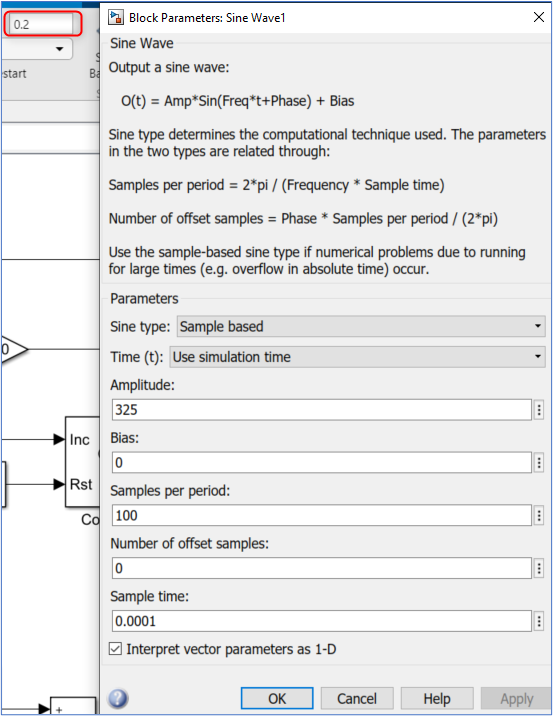
\includegraphics[width=\linewidth]{Bilder/Lauferkennung_Peaks_SinusSignalGenerator.png}
	\caption{Testbeispiel - Lauferkennung - Sinussignalgenerator - Spezifikationen}
	\label{fig:Lauferkennung_Peaks_SinusSignalGenerator}
\end{figure}
Eine zeitliche Frequenz wird folgendes berechnet:
$Freq(Hz) = Freq(rad/sec) / (2 * pi)$; $pi = 3,14$
\begin{figure}[H]
	\centering
	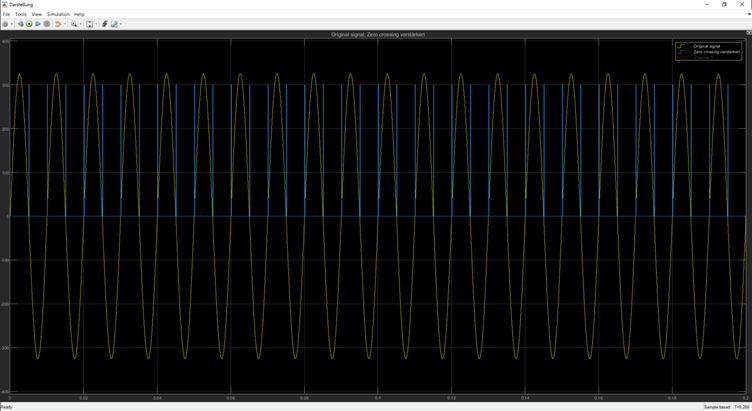
\includegraphics[width=\linewidth]{Bilder/Lauferkennung_Peaks_SinusSignal.png}
	\caption{Testbeispiel - Lauferkennung - Sinussignal}
	\label{fig:Lauferkennung_Peaks_SinusSignal}
\end{figure}
\autoref{fig:Lauferkennung_Peaks_SinusSignal} zeigt die Ausgabe der Scope-Funktion. In der Grafik ist das generierte Sinussignal (gelb) sowie wie of das Signal die Nulllinie überschneidet (blau).
In der Scope-Darstellung sind das originale Sinussignal und ein Zähler sichtbar. Der Zähler hat jeden ‚Zero-crossing‘ aufgezählt.
Das Testmodell hat die richtige (erwartete) Ergebnisse geliefert: 100 Hz als Frequenz.
Beim Einsetzen des gleichen Vorgehens auf das richtige Signal ($AccBfX_mg$) (das kalibrierten Signal) wurde eine Frequenz von ca. $11$ Hz beim Laufen und eine Frequenz zwischen $20-30$ Hz ausgerechnet. Das hat die Erwartungen nicht entsprochen.
Daraus kann folgendes extrahiert werden:
Beide Signale (Szenarien) (Laufen und Fahren) haben die gleiche Menge von Störungen (Rauschen). Der Unterschied ist die Amplitude. Es kann keine Amplitude ‚Hartkodiert‘ entdeckt werden, da die Amplitude sich ständig ändern kann.
************ Grafiken von den zwei Signalen darstellen und die Art der Rauschen näher analysieren (was könnte die Ursache sein?); Welche mögliche Lösungen gäbe es dafür? *************\\

.\\

\textbf{Ergebnis: Die Frequenz muss allerdings doch gesucht und schließlich verglichen werden}




\subsection{Frequenzbasierend} %TODO: ausführlich beschreiben
Auf die FFT beziehen.\\

zum Berechnen der Frequenz: FFT (Fast Fourier Transformation)\\

Nochmal das gleiche mit dem Testmodel durchgeführt.\\


\begin{figure}[H]
	\centering
	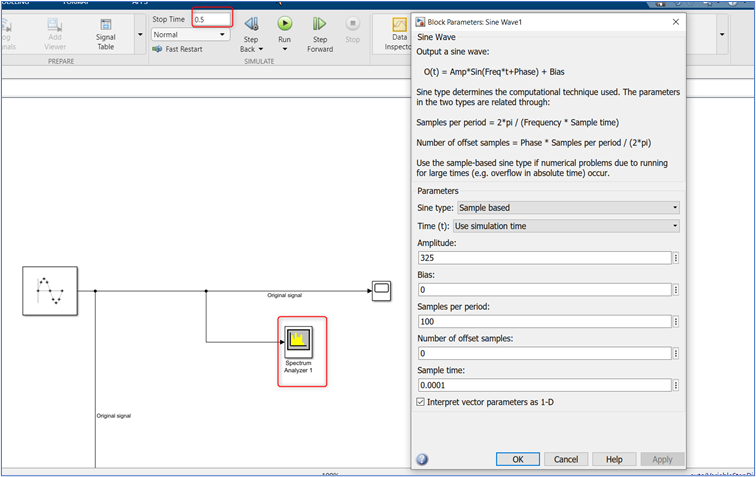
\includegraphics[width=\linewidth]{Bilder/Lauferkennung_Freqbasiert_TestBeispiel_SinussignalGenerator.png}
	\caption{Testbeispiel - Frequenzbasierte Lauferkennung - Sinussignal}
	\label{fig:Lauferkennung_Freqbasiert_TestBeispiel_SinussignalGenerator}
\end{figure}

\begin{figure}[H]
	\centering
	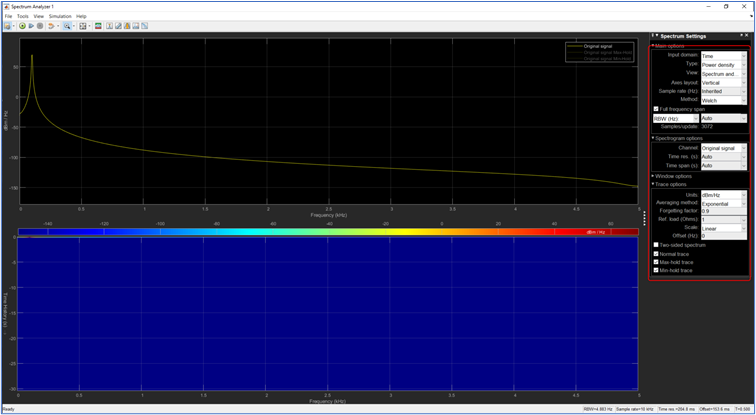
\includegraphics[width=\linewidth]{Bilder/Lauferkennung_Freqbasiert_SpektrumAnalyzerAusgabe.png}
	\caption{Testbeispiel - Frequenzbasierte Lauferkennung - Ausgabe des Spektrum-Analyzer und seine Spezifikationen}
	\label{fig:Lauferkennung_Freqbasiert_SpektrumAnalyzerAusgabe}
\end{figure}

\begin{figure}[H]
	\centering
	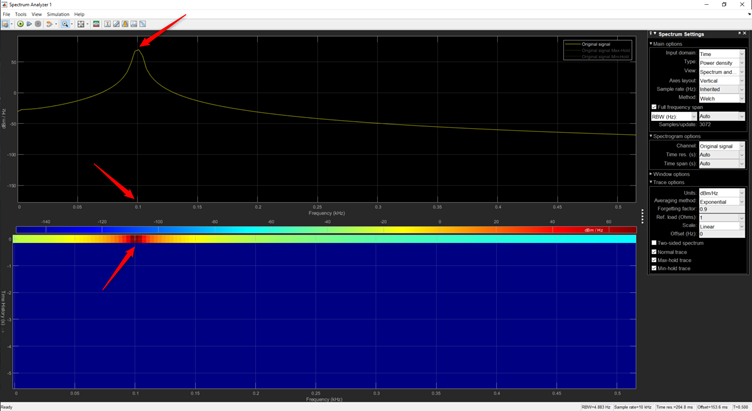
\includegraphics[width=\linewidth]{Bilder/Lauferkennung_Freqbasiert_SpektrumAnalyzerAusgabe_gezoomt.png}
	\caption{Testbeispiel - Frequenzbasierte Lauferkennung - Ausgabe des Spektrum-Analyzer im Bereich zwischen 0-0.5 kHz}
	\label{fig:Lauferkennung_Freqbasiert_SpektrumAnalyzerAusgabe_gezoomt}
\end{figure}

\autoref{fig:Lauferkennung_Freqbasiert_SpektrumAnalyzerAusgabe_gezoomt} Es ist schön zu bemerken, dass die Frequenz (100 Hz) sehr gut sichtbar ist. Der obere Teil zeigt die Häufigkeit einer Frequenz (Spektrum) unabhängig von der Zeit. Der untere Teil zeigt die Häufigkeit einer Frequenz mit der Zeit (Spektrogramm).

\begin{figure}[H]
	\centering
	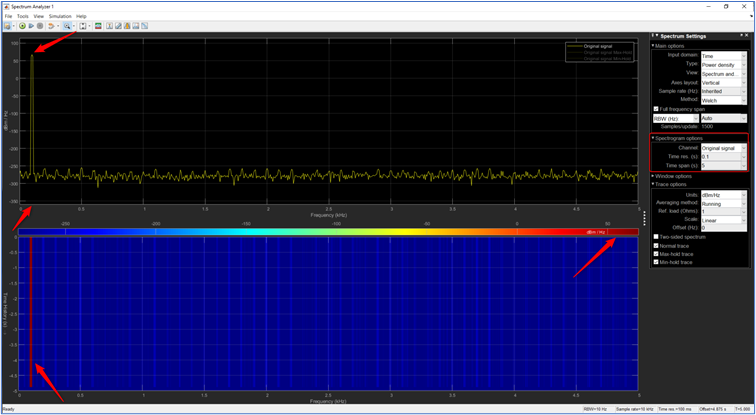
\includegraphics[width=\linewidth]{Bilder/Lauferkennung_Freqbasiert_SpektrumAnalyzerAusgabe_2Einstellungen.png}
	\caption{Testbeispiel - Frequenzbasierte Lauferkennung - Ausgabe des Spektrum-Analyzer mit anderen Spezifikationen}
	\label{fig:Lauferkennung_Freqbasiert_SpektrumAnalyzerAusgabe_2Einstellungen}
\end{figure}

\begin{figure}[H]
	\centering
	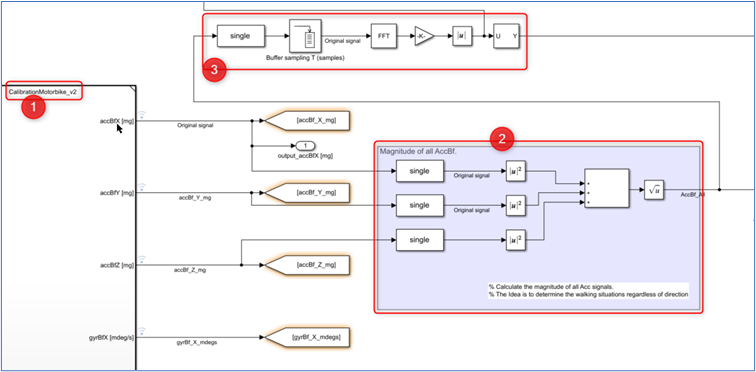
\includegraphics[width=\linewidth]{Bilder/Lauferkennung_Freqbasiert_FFT.png}
	\caption{Testbeispiel - Frequenzbasierte Lauferkennung - FFT - Modell}
	\label{fig:Lauferkennung_Freqbasiert_FFT}
\end{figure}

Die AccBfX, AccBfY und AccBfZ sind die Ausgänge des Modells $CalibrationsMotorbike_V2$ und sie sind die Kalibrierte Signale.
Diese Werte werden für die Berechnung der Betrag mit der Formel (**********************)
%TODO: $AccBf_All=√(〖AccBfX〗^2+ 〖AccBfY〗^2+〖AccBfZ〗^2 )$ 
verwendet (\autoref{fig:Lauferkennung_Freqbasiert_FFT}- Nummer 2). Das Ziel ist die Frequenzermittlung richtungsunabhängig zu stellen.
Danach wurde eine FFT an der Variablen $AccBf_All$ durchgeführt, um die Frequenzen zu ermitteln (\autoref{fig:Lauferkennung_Freqbasiert_FFT}- Nummer 2).


\begin{figure}[H]
	\centering
	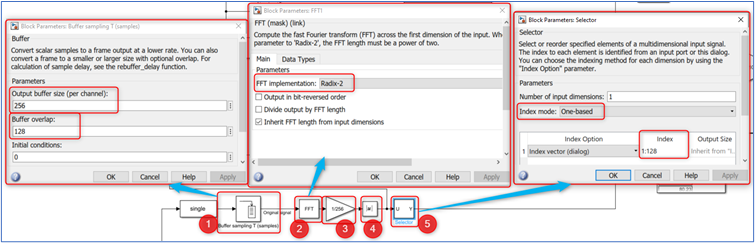
\includegraphics[width=\linewidth]{Bilder/Lauferkennung_Freqbasiert_FFT_Spezifikationen.png}
	\caption{Testbeispiel - Frequenzbasierte Lauferkennung - FFT - Modell}
	\label{fig:Lauferkennung_Freqbasiert_FFT_Spezifikationen}
\end{figure}
In der \autoref{fig:Lauferkennung_Freqbasiert_FFT_Spezifikationen} wird eine FFT durchgeführt. Die Einstellparameter jedes Element ist ersichtlich.

1-	In der Buffer sind 256 Samples zu betrachten (d.h. ca. 2,5 Sekunden des Signals, da die Abtastrate der Sensor 100 Hz ist). Eine Überlappung von ca. 1 Sekunde wurde auch eingestellt, damit die Zwischen Frequenzen nicht übersehen werden.\\
2-	Der FFT-Typ ist eine Radix-2.\\
3-	Die Ausgabenwerte der FFT durch 265 dividieren. (warum?)\\ %TODO: warum 
4-	Betrag des FFT-Ausgangs bilden (warum?)\\ %TODO: warum 
5-	Da FFT ein gespiegelter Ausgang liefert wird nur die Hälfte der Matrix angenommen (1:128)\\
\subsubsection{Entscheidungskriterien - Matlabskript}
%
%
%
%
%
Screenshot vom Skript mit einer Erklärung (\autoref{fig:MatlabSkript}) %TODO: Skript erklären und eine Ablaufschema (Entscheidungsbaum) erstellen
\begin{figure}[H]
	\centering
	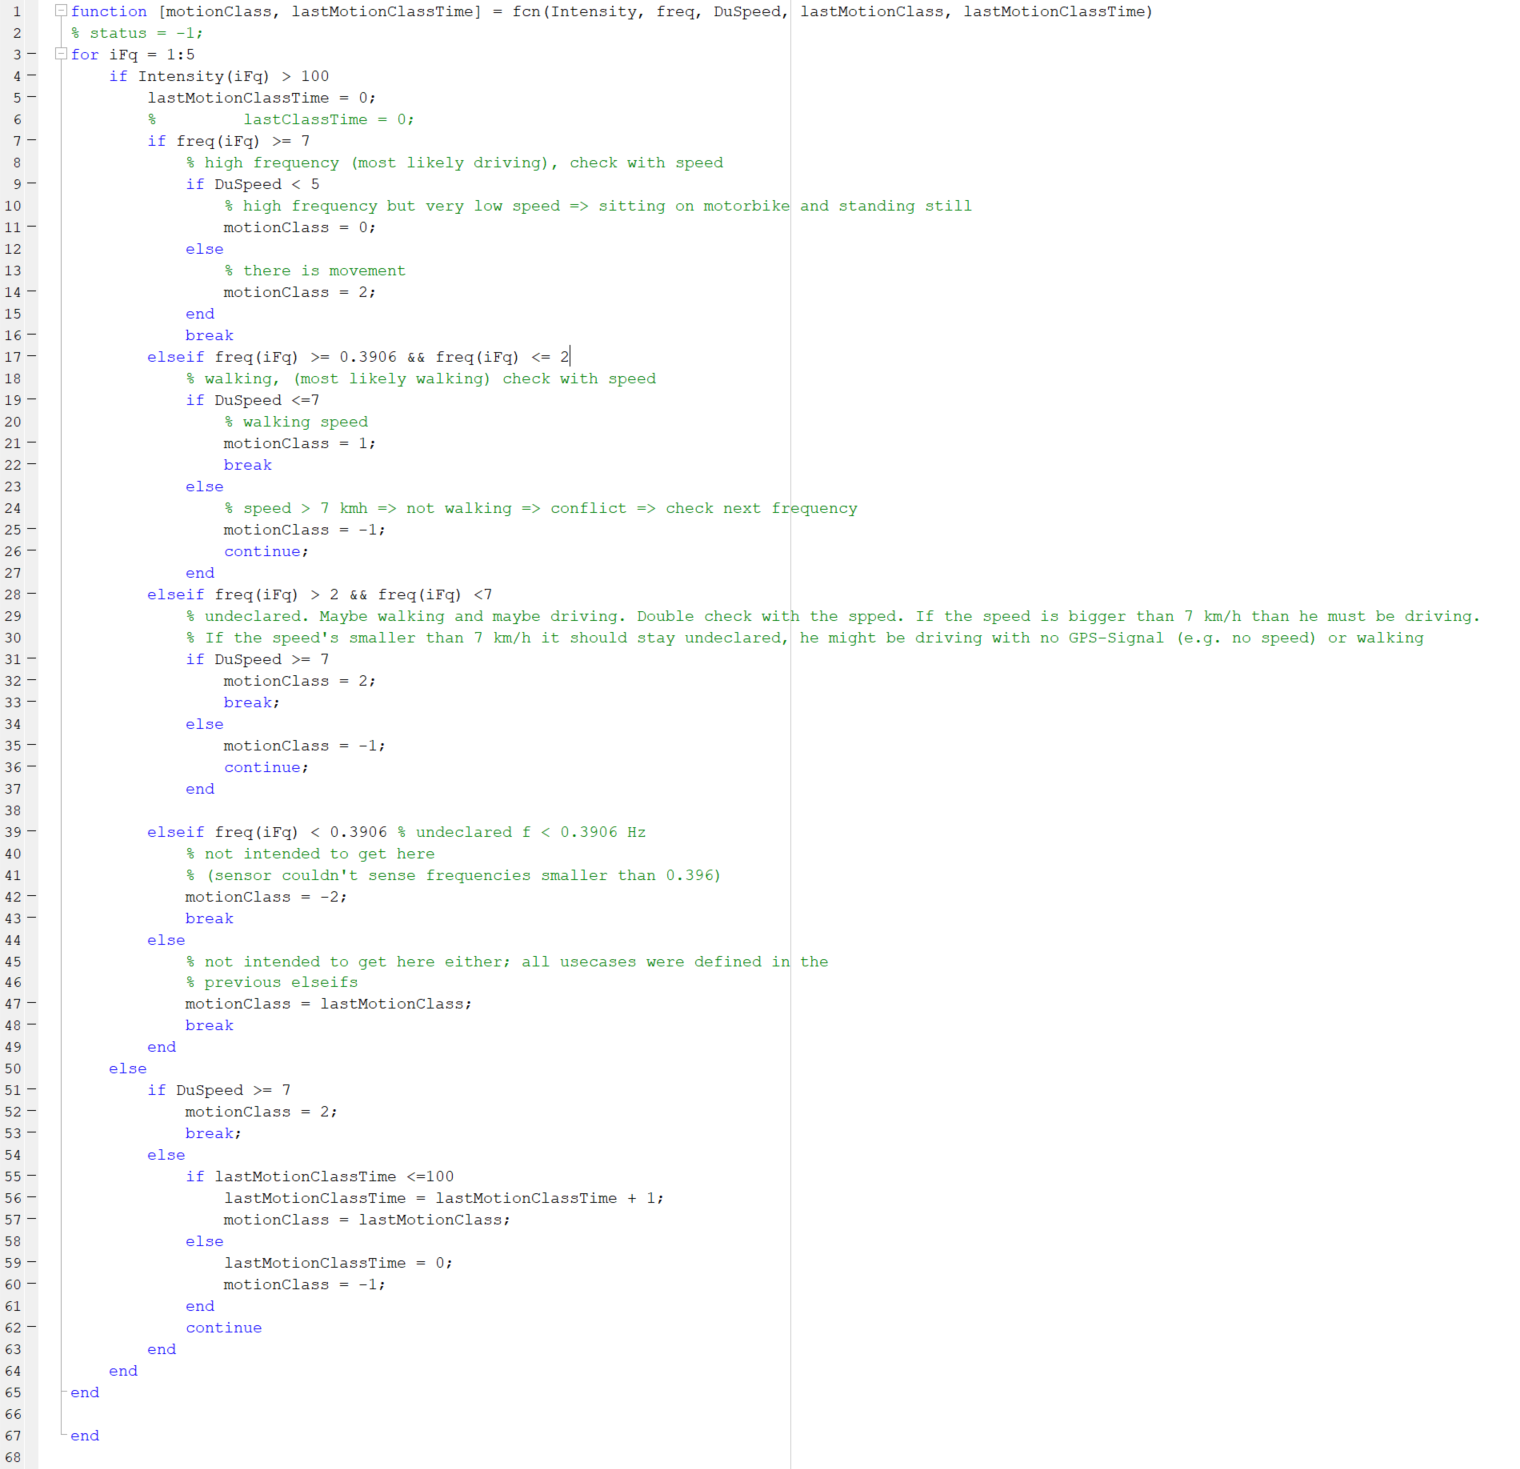
\includegraphics[width=\linewidth]{Bilder/MatlabSkript.png}
	\caption{Entscheidungsskript durch mehrere Kriterien (Frequenz und Geschwindigkeit)}
	\label{fig:MatlabSkript}
\end{figure}




\subsubsection{Beispiel}
Mögliche Konflikte: ID = 2488; CrashNoPSAP;\\

\begin{figure}[H]
	\centering
	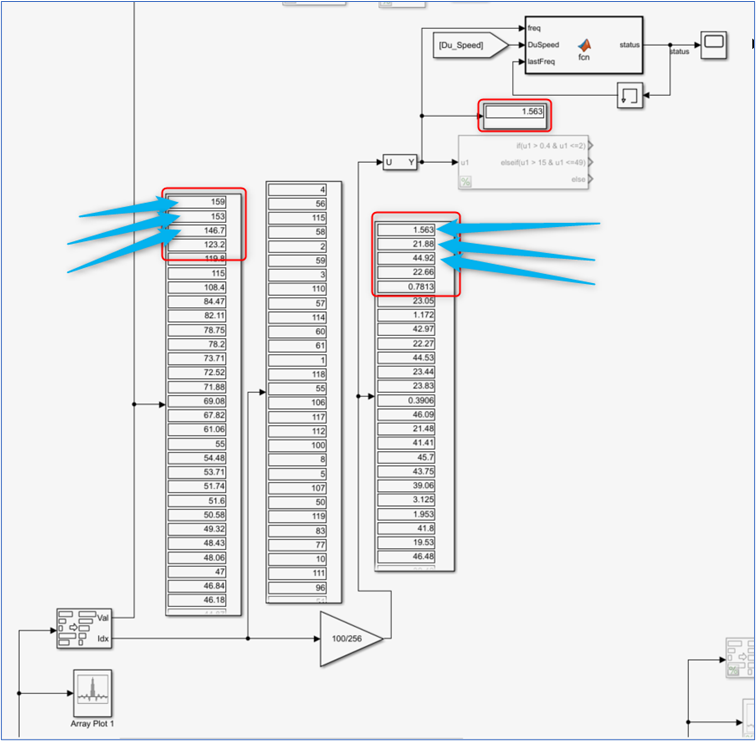
\includegraphics[width=\linewidth]{Bilder/Lauferkennung_Freqbasiert_Ausgangsbeispiel.png}
	\caption{Testbeispiel - Frequenzbasierte Lauferkennung - Ausgangsbeispiel - ID 2488}
	\label{fig:Lauferkennung_Freqbasiert_Ausgangsbeispiel_ID2488}
\end{figure}
Da hier (\autoref{fig:Lauferkennung_Freqbasiert_Ausgangsbeispiel_ID2488} und \autoref{fig:Lauferkennung_Freqbasiert_Ausgangsbeispiel_ID2488_Scope}) die maximale Intensität der Frequenz 1,5, wird diese als das Maximum übernommen und weiterbearbeitet. Die nächste größte Intensität liegt sehr nah dazu und hat die Frequenz 21,88 Hz, was eigentlich richtiger ist.

\begin{figure}[H]
	\centering
	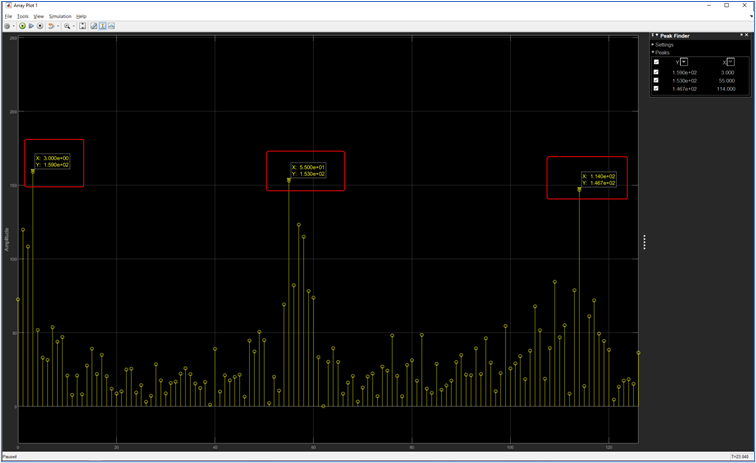
\includegraphics[width=\linewidth]{Bilder/Lauferkennung_Freqbasiert_Ausgangsbeispiel_ID2488_Scope.png}
	\caption{Testbeispiel - Frequenzbasierte Lauferkennung - Ausgangsbeispiel - ID 2488 - Scope}
	\label{fig:Lauferkennung_Freqbasiert_Ausgangsbeispiel_ID2488_Scope}
\end{figure}




\subsubsection{Werte Sinnvoll auswählen}
- gültige Intensität\\
- Frequenzbereiche\\
- Gültige Geschwindigkeit\\
- Ausschlusskriterien\\





\section{Verifikation des Algorithmus'}
% Aufgrund der Verifizierung des Algorithmus werden im Folgenden statistische Zahlen über Fahrradunfälle weltweit sowie in Deutschland dargestellt. Danach wird eine statistische Fallzahlabschätzung durchgeführt, um die notwendige Anzahl der Versuche zu ermitteln. Eine Versuchsplannung wird anhand der Ergebnisse der Versuche durchgeführt, die bereits vor der eigentlichen Verifizierung durchgeführt wurden. 
%
%
%


\subsection{Groundtruth sammeln}

- Videos mit den Daten synchronisieren (Das Tool erläutern? oder vllt. nur erwähnen?)\\
- Groundtruth labels nachdenken und erläutern\\
- Videos labeln\\

















